\documentclass[conference]{IEEEtran}
\usepackage{times}

% numbers option provides compact numerical references in the text.
\usepackage[numbers]{natbib}
\usepackage{multicol}
\usepackage[bookmarks=true]{hyperref}

\usepackage{amsmath}
\usepackage{amssymb}
\usepackage{amsthm}
\usepackage{bm}
\usepackage{dsfont}
\usepackage{graphicx}

\pdfinfo{
   /Author (Alvin Sun)
   /Title  (Robots: Our new overlords)
   /CreationDate (D:20101201120000)
   /Subject (Robots)
   /Keywords (Robots;Overlords)
}


\begin{document}

% paper title
\title{Learning Continuous Contact Dynamics from Vision}

% You will get a Paper-ID when submitting a pdf file to the conference system
%\author{Author Names Omitted for Anonymous Review.}

\author{\authorblockN{Alvin Sun}
\authorblockA{Department of Mechanical Engineering\\
Stanford University\\
Stanford, California 94305\\
Email: alvinsun@stanford.edu}}

\maketitle

\begin{abstract}
  Dynamical system identification has always been a core component in deriving
  high-performance robust controller that requires long-horizon predictive models.
  While various model learning successes were achieved,
  obtaining contact dynamics remains one of the most challenging and unsolved
  problems that are also crucial for a wide range of manipulation tasks. We
  propose to research on a self-supervised learning method that explicitly
  exploits the switching structure of contact dynamics in a latent coordinate
  space generated through vision. Taking advantage of the increasingly popular
  neural ODE \cite{neural_ode}, this proposal has the potential of learning a
  continuous contact dynamical model that is capable of long-horizon forward prediction without
  intermediate visual measurements. This will further make achieving high precision
  contact manipulation possible with optimal controllers such as MPC
  implemented in the latent space.
\end{abstract}

\IEEEpeerreviewmaketitle

\section{Introduction}
Precise manipulation of objects, especially in
unknown environment, has long been a challenging problem that is preventing
autonomous robot manipulators from reaching the intelligence of a human.
There are several difficulties:
\begin{enumerate}
  \item Computing for the dynamics of the manipulator alone could sometimes be
    quite difficult considering the number of DOF it could have. This is especially
    true if the manipulator is deployed to mobile platforms where the true
    state of the platform itself is hard to estimate.
  \item The surrounding environment, even though for the non interacting part,
    is hard to model, given it can potentially include an infinite number of
    possible configurations.
  \item Most importantly, precise manipulation of objects require some knowledge
    of the object itself -- either its physical dynamics or its states.
    However, the object(s) of interests, or the ones to be manipulated,
    has physical properties that are most of the time unknown to the manipulator.
    Many commonly seen objects could even be deformable, of which the dynamics
    are even harder to learn.
\end{enumerate}

Human naturally deal with such challenges with feedback. The control policy gets
adjusted on the fly when a human approaches some objects and potentially makes
mistakes such as misalignment or grasp inaccuracy. Vison, tacile, and proprioception
are the main sensory feedbacks that aid humans to achieve such adjustment. However,
to utilize all those sensory feedback, from a dynamical system perspective,
manipulation is not only about knowing the dynamics
of the actuation, but also about estimating the dynamics of the object to be
manipulated. Manipulation dynamics can be thought as changing
the states of both the manipulator and the objects with some actions.
As pointed out by \citet{imitation},
the learning process of human infant rely heavily on visual
perception, which implies that visual information is quite rich in
encapsulating interactive manipulation dynamics. In fact, a video stream, or
a temporal sequence of images, contains the complete information about where
things are and how fast things are moving, which is basically the laws of physics.

Therefore, we would take inspiration
from such intuition and propose a vision based learning method
for contact dynamics identification that can be useful for a wide range of
manipulation tasks. More specifically, we propose a self-supervised
learning method for obtaining joint visual representation of the dynamics of both
the manipulator and the environment it is interacting with. In control
literature, real-world dynamical system is usually modeled with
\begin{gather}\label{eqa:dynamic_cont}
  \dot{x}(t) = f(x(t), u(t)),
\end{gather}
while sometimes discretized to the form
\begin{gather}\label{eqa:dynamic_disc}
  x_{k+1} = f(x_k, u_k).
\end{gather}
Our method is effectively a forward predictive model in the form of
Equation~\ref{eqa:dynamic_cont} where the encoded states $x$ encapsulate both the
manipulator as well as the object it is trying to manipulate. This learned
dynamics can be integrated for more efficient downstream tasks such as
control optimization that takes the manipulated object into account.

\section{Background}

\subsection{Modeling ODEs with Neural Nets}\label{sec:neural_ode}
It is very common and general to model real-world dynamical systems with
first-order ODEs in the form of
Equation~\ref{eqa:dynamic_cont}, and this has led to a lot of efforts in
bringing in machine learning tools to estimate such continuous dynamical
given the excellent function approximation capabilities of neural nets.
\citet{neural_ode} has presented a breakthrough technique that allows modeling
the dynamical functions $f$ as parameterized neural networks. This has
become increasingly popular in a wide range of settings involving dynamical systems.
One of the main contribution of this work is deriving a computationally feasible algorithm
for gradients backpropagation through ODE solvers. Here I will give a quick
overview of how gradients are computed for numerically solved ODEs. Consider
the more general (than Equation~\ref{eqa:dynamic_cont}) form below,
\begin{gather}
  \dot{x} = f_\theta(x, t).
\end{gather}
This ODE can be solved with any generic ODE solver as follows
\begin{align}
  x(t) &= x(t_0) + \int_{t_0}^{t} f_\theta(x(\tau), \tau) d\tau \\
       &= \text{ODESolve}(f_\theta, x(t_0), t_0).
\end{align}
Usually, we are interested in a loss function, $\mathcal{L}(x(t))$, which
takes those integrated states into account. In order to learn, we will have
to compute the gradients with respect to both the dynamical parameters $\theta$
and the states $x(t)$. We first define an adjoint state $a(t)$,
\begin{gather}
  a(t) = \frac{\partial \mathcal{L}}{\partial x(t)}.
\end{gather}
It can then be proven (see Appendix in \cite{neural_ode}) that the adjoint states
themselves satisfy another set of ODEs,
\begin{gather}
  \frac{da(t)}{dt} = -a(t)^T \frac{\partial f_\theta(x(t), t)}{\partial x(t)}.
\end{gather}
Finally, the gradient with respect to $\theta$ is yet another ODE,
\begin{gather}
  \frac{d}{dt}\left(\frac{\partial \mathcal{L}}{\partial \theta}\right) =
  a(t)^T \frac{\partial f_\theta(x(t), t)}{\partial \theta}.
\end{gather}
The authors have also shown that all those ODEs can be vectorized into one
single call to an ODE solver that generates the necessary gradients for
$\theta$ as well as the intermediate states $x(t)$. This technique is crucial
for our proposed continuous dynamical model to learn from data.

\subsection{Dynamic Object Segmentation}\label{sec:object_seg}
For object manipulation tasks concerning vision inputs, it is crucial for the
vision pipeline to have the capabilities of segmenting the objects out.
\citet{3d_detection} presented a powerful method to do such segmentation
by comparing differences between different point clouds. The general idea of
their algorithm consists of two steps:
\begin{enumerate}
  \item Compute a set of points that is present in either of the two aligned
    point clouds but not both.
  \item Filter this set of points by first removing small clusters
    (that mostly consist of noise), and then retaining the clusters of points that
    occupy the free space in the other point clouds.
\end{enumerate}
This is really useful for many manipulation settings, as the manipulator has a
relatively confined workspace, which can be scanned beforehand. Using that
pre-scanned map, and any real-time inference point clouds, we can easily segment
out the objects using this dynamic object segmentation method.

\section{Related Work}

\subsection{Model Learning}
The learning of unknown dynamics, also known as the system identification
problem, has been tackled from a wide range of angles. Dynamic Mode Decomposition
\cite{dmd} and its nonlinear variant eDMD \cite{edmd} are two of the most
widely applied system identification approaches that exploited the eigen
structures of (locally) linear dynamical systems. Later, \citet{dmdc} applied
control algorithms to models learned from DMD.
More recently, \citet{sindy} proposed to SINDy, which utilizes compressed
sensing techniques
to learn the true underlying physics of arbitrary dynamical systems by getting
a sparse set of coefficients for a large non-linearity dictionary. \citet{sindyc}
later applied model predictive control on systems identified using SINDy.
\citet{deepsindy} built on top of SINDy and use deep neural networks to
generalize for high dimensional inputs such as images. However,
for all of the methods mentioned, the learned models are mostly for
standalone dynamics that do not account for complicated interactions
such as contact.
In the RL literature, \citet{pilco} proposed to model arbitrary unknown
(discrete) dynamical model following Equation~\ref{eqa:dynamic_disc}
as Gaussian processes. Though it resulted in data-efficient learning of a wide range
of systems, it again does not consider any dynamic interaction with the
environment. \citet{deeppilco} later generalizes this method to work with
high dimensional image spaces, but still does not concern interaction.

\subsection{Visual Representation}
\citet{deep_visuomotor} started the area on visuomotor learning with an end-to-end
learning algorithm for manipulation tasks. However, the learning process relies on a local
controller that has full observability over the states of the object. Several
methods \cite{latent_dynamics, dream_to_control} explicitly learn latent dynamics
of the environment, but without exploiting the structure of the switching dynamics
for contact situations. \citet{dense_objnet} have come up with
explicit dense visual representations of the environment, but the connection of
those learned representations to manipulation policies is unclear. \citet{vision_touch}
on the other hand, presented a self-supervised method for generating representations
that fuse multiple sensor modalities including vision. The learned representation
is then fed as input to a model-free reinforcement algorithm to generate the
control policies. Even though some dynamical information is definitely encoded
in those representations, there is no explicit way to predict long-term dynamical evolution
from those representations, which limits their ability to incorporate any
high-performance model-based controller. \citet{dense_physics} propose to explicitly learn the
physics of real-world items through programmed interactions, but its push-then-observe
formulation is fairly limited to just estimating the inertia properties of the objects
rather than achieving continuous contact manipulation.

\section{Proposed Research}
\subsection{Problem Formulation}
We propose a self-supervised vision-based learning method for estimating joint
dynamical representation of the robotic manipulator as well as the objects to be manipulated.
Considering the causal effect between the control inputs and states, some control input
could cause some states (sometimes both the manipulator and the objects) to change.
The change is reflected in the direction of motion, which is the time derivative
term in Equation~\ref{eqa:dynamic_cont}. However, during the reaching phase of
manipulation, when the manipulator is not in contact with the object, it is
unlikely that the action of the manipulator could cause a state change of an
object unless there are external interaction among the environments. If
we use $x_m$ and $x_e$ as the states of the manipulator and environment
respectively, and $u$ as the action for the manipulator, we can first
create a contact detector model $c$ such that
\begin{gather}
  c(x_m, x_e) = \mathds{1}\{\text{$x_m$ and $x_e$ is in contact}\}.
\end{gather}
Then we can formulate an explicit switching dynamics for both the manipulator
and the environments,
\begin{equation}
  \begin{aligned}
    \dot{x}_m &= \begin{cases}
      f_m^{\bar{c}}(x_m, u) & \text{if $c(x_m, x_e) = 0$} \\
      f_m^c(x_m, x_e, u) & \text{otherwise}
    \end{cases}\\
    \dot{x}_e &= \begin{cases}
      f_e^{\bar{c}}(x_e) & \text{if $c(x_m, x_e) = 0$} \\
      f_e^c(x_m, x_e, u) & \text{otherwise}
    \end{cases}
  \end{aligned}
\end{equation}
However, this switching formulation can be really hard to learn as this
introduces some discontinuity to the overall dynamical system. Taking the
analogy from Residual Policy Learning \cite{residual_policy}, we can re-formulate
the dynamical system with two parts: a canonical non-contact dynamics and a
residual contact dynamics,
\begin{equation}\label{eqa:soft_dyn}
  \begin{aligned}
    \dot{x}_m &= f_m(x_m, u) + c(x_m, x_e) \cdot r_m(x_m, x_e, u) \\
    \dot{x}_e &= f_e(x_e) + c(x_m, x_e) \cdot r_e(x_m, x_e, u)
  \end{aligned}
\end{equation}
where $f_m$ and $f_e$ are the canonical non-contact dynamics and $r_m$ and
$r_e$ are the residual contact dynamics that compensate for contact corrections.
This re-formulation not only makes the residual dynamics easier to learn as
compared to the full complicated contact dynamics but also makes the full
dynamical system differentiable due to its soft-switching structure.
Now, given all those canonical / residual dynamics are unknown, and the
inputs are high dimensional, we would need a compressed latent representation
of the dynamics.

\subsection{Modeling with Deep Neural Networks}
\begin{figure*}[hbt]
  \centering
  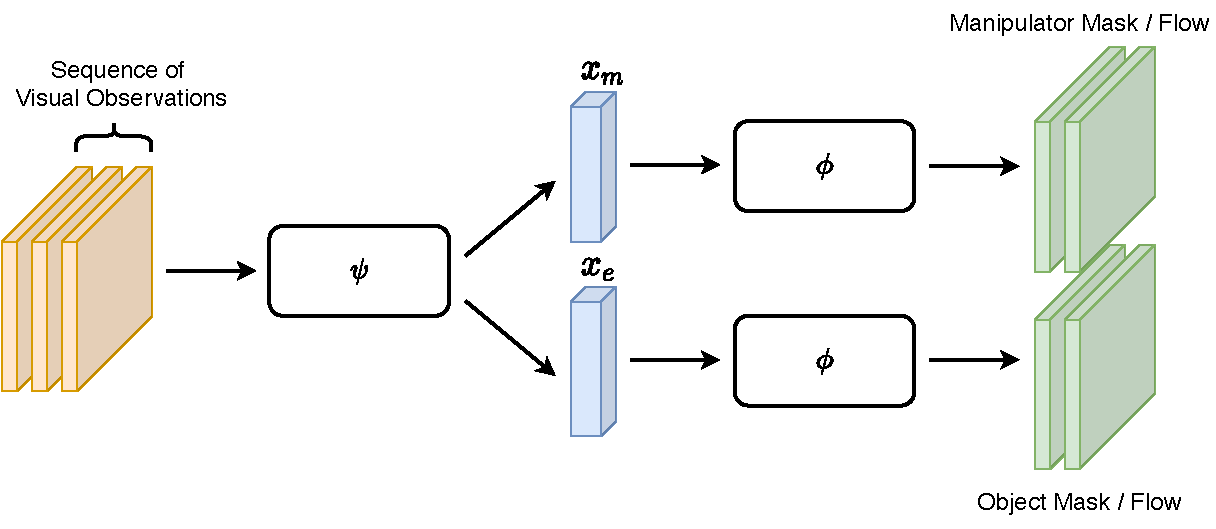
\includegraphics[width=.7\textwidth]{model_arch_ae}
  \caption{Latent Coordinates Extraction from Convolutional Autoencoder}
  \label{fig:model_ae}
\end{figure*}
\begin{figure}[hbt]
  \centering
  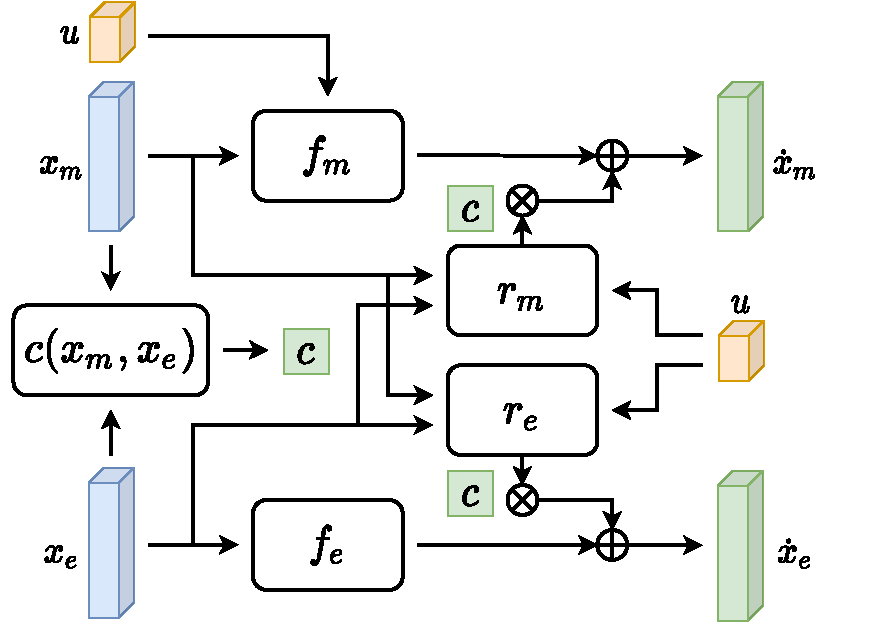
\includegraphics[width=.48\textwidth]{model_arch_dyn}
  \caption{Contact Residual Dynamics}
  \label{fig:cont_dyn}
\end{figure}
As we propose to infer state information from pure vision data, we require the inputs
to contain full state information including the derivates such as velocities. As a
result, the inputs from which we are extracting a latent representation consist of
a sequence of $K$ images. In our proposal pick any $K \ge 3$ should be sufficient
to infer the full dynamical information purely from images. Let $\mathcal{I}$ denote the
sequence of input images, we can learn the latent dynamics with a convolutional
autoencoder network, with encoder $\psi$ and decoder $\phi$, where
\begin{gather}
  \begin{bmatrix}x_m \\ x_e\end{bmatrix} = \psi(\mathcal{I}).
\end{gather}
The dynamical information in the image space, intuitively, is just the location
and rate of movement of both the manipulator and the environment (or the object
to be manipulated). Those can be encoded as a segmentation mask, $I^s$, and an optical
flow image, $I^f$. To enforce that the latent dynamics contain the necessary dynamical
information, we will have the decoder to generate those image space dynamics
as follows
\begin{equation}
  \begin{aligned}
    \begin{bmatrix}\hat{I}_m^s \\ \hat{I}_m^f\end{bmatrix} &= \phi(x_m) \\
    \begin{bmatrix}\hat{I}_e^s \\ \hat{I}_e^f\end{bmatrix} &= \phi(x_e)
  \end{aligned}
\end{equation}
The decoder weights are shared for both the manipulator states and the object states
since we don't want the encoder to implicitly distinguish between manipulator and
objects from the image which can cause overfitting problems. This will ensure
that the latent dynamical structures are similar for the two states.
An overview of the autoencoder architecture is shown in Figure~\ref{fig:model_ae}.
The supervision training signal will be provided by minimizing the reconstruction error
between the decoded outputs and the ground truth mask and flow for both the manipulator
and the objects. Here we can define the loss for segmentation reconstruction as a
standard cross-entropy loss,
\begin{gather}\label{eqa:loss_seg}
  \mathcal{L}^s = I^s \cdot \ln(\hat{I}^s) + (1 - I^s) \cdot \ln(1 - \hat{I}^s).
\end{gather}
For the flow reconstruction loss, we use the standard mean square error but
masked by the segmentation, i.e.
\begin{gather}\label{eqa:loss_flow}
  \mathcal{L}^f = \|I^s \cdot (I^f - \hat{I}^f)\|^2.
\end{gather}
Those two losses in Equations~\ref{eqa:loss_seg} and \ref{eqa:loss_flow} apply to
both the decoded manipulator states and decoded object states.
The generation of those ground true images is discussed in further
details in Section~\ref{sec:data_gen}.
The contact model, $c(x_m, x_e)$, can also be learned as a binary classifier
again using the standard cross-entropy loss,
\begin{gather}
  \mathcal{L}^c = c \cdot \ln(\hat{c}) + (1 - c) \cdot \ln(1 - \hat{c}),
\end{gather}
where the ground truth contact indicator can be generated through force / torque
sensor readings.

As for the contact residual dynamics, an overview of its architecture is shown in
Figure~\ref{fig:cont_dyn}, and all of those dynamical subcomponents, $f_m$, $f_e$,
$r_m$, and $r_e$, are modeled with MLPs (multi-layer perceptron), which are known
to have very good function approximation capabilities.
Even though this representation learns a structured
continuous dynamical model in the latent space, Equation~\ref{eqa:soft_dyn} can
still be viewed as a general dynamical ODE in the following form,
\begin{gather}\label{eqa:joint_dynamics}
  \dot{x} = \begin{bmatrix}\dot{x}_m \\ \dot{x}_e\end{bmatrix} = f(x, u),
\end{gather}
where all the contact detector and soft switching logic is baked into $f$.
We can then use it to rollout longer horizon trajectories with ODE integration,
\begin{gather}
  \hat{x}(t) = \text{ODESolve}(f, x(t_0), t_0).
\end{gather}
The final loss for learning this latent dynamical evolution is then to regress
on the rolled-out trajectories with the actual trajectories,
\begin{gather}
  \mathcal{L}^d = \|x(t) - \hat{x}(t)\|^2,
\end{gather}
where $x(t) = [x_m(t), x_e(t)]^T$ is generated by the encoder network directly
on the sequences of images at time $t$.
All gradients computation can be achieved as discussed in
Section~\ref{sec:neural_ode}.
The overall loss for training everything jointly is then
\begin{gather}
  \mathcal{L} = \mathcal{L}_m^s + \mathcal{L}_e^s + \mathcal{L}_m^f + \mathcal{L}_e^f +
                \mathcal{L}^c + \mathcal{L}^d.
\end{gather}

\subsection{Experiment Setup}
\begin{figure}[hbt]
  \centering
  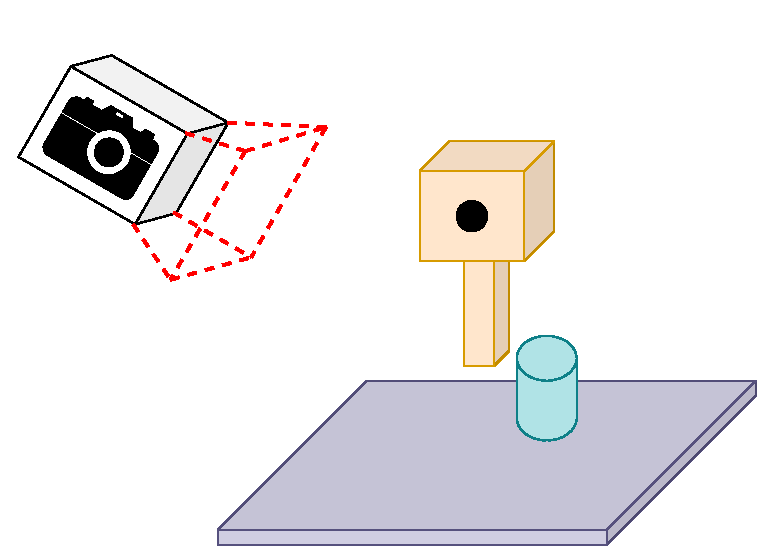
\includegraphics[width=.45\textwidth]{experiment}
  \caption{Illustration of an Experiment Setup}
  \label{fig:exp_setup}
\end{figure}
We propose to set up a preliminary experiment with a relatively simple but
contact-rich manipulation scenario. Figure~\ref{fig:exp_setup} illustrates
how sensors and actuators are involved in the proposed experiments. For the
actuators, we proposed to use a 5D push manipulator with actuated pendulum-like
dynamics. This manipulator has 3 DoFs for translation in free space, 1 DoF in
rotation about the upright axis, and 1 DoF for controlling the pendulum finger.
This setup contains simple canonical dynamics but also encourages learning
of dexterous contact behaviors with finger motions.

For the sensors, the primary sensory system for our proposed method is vision,
which requires an RGBD camera with a fixed viewing position. With this configuration,
a pre-scan of the manipulation workspace can be done beforehand, and then
the objects can be dynamically segmented out in real-time with methods discussed
in Section~\ref{sec:object_seg}. Force / torque sensor will also be installed
on the pendulum arm primarily for contact detection.

\subsection{Automatic Data Generation}\label{sec:data_gen}
To avoid tedious process of manually labeling the datasets which can also prone to
human errors, our proposed method
generates ground truth data in a self-supervised manner. Two of the most challenging labels
to generate are the ground truth mask and flow for both the manipulator and the
objects. For the manipulator, those data are not as hard to generate since the
robotic manipulator has known proprioception, and in combination with the
known camera calibration, we can project the known manipulator states to the camera
frame to generate the ground truth mask and flow. On the other hand, generating
mask and flow images for arbitrary objects is a little more tricky. Thanks to \cite{3d_detection},
we can segment out the object in real-time by comparing the difference of the
point cloud generated through the RGBD sensor and a pre-scanned point cloud
of the workspace. Backprojection of the point cloud segmentation gives the
image space segmentation for the object. As for generating the ground truth
flow, additional steps are required. We first need to compute the relative
transform of the object from frame to frame. This can be done with the iterative
closest point (ICP) algorithm on the segmented object point cloud. It is reasonable
to assume that this can be achieved in real-time since the set of points belonging
to an object is relatively small. We can then estimate the velocity of movement
via finite differencing. Backprojecting the velocity vectors of each point
gives the flow vector in image space. The last label that needs to be generated
is the contact indicator. Since we have force / torque sensor installed on the
manipulator finger, this can easily be done via simple thresholding on the
force / torque readings.

\subsection{Evaluation Metrics}
The primary goal of this proposal is to learn an accurate latent contact dynamical
model that is capable of performing long-horizon prediction, so the main evaluation
metric is constructed to verify the quality of the model prediction.
One direct number we can use is the dynamical rollout loss, which indicates how
well can the latent trajectories be predicted without any visual measurements.
Another metric we can use is the reconstruction error on the rolled out trajectories.
Namely, this is the difference between the ground truth mask and flow and
$\phi(\hat{x}_m)$ and $\phi(\hat{x}_e)$, where $\hat{x}_m$ and $\hat{x}_e$ come
from the dynamical rollout of some finite horizon. This metric describes how
well the dynamical hallucination matches reality.

To verify the effectiveness of explicitly exploiting the contact structure with
this gated residual representation, a baseline approach can be constructed by
modeling everything with a joint dynamical model as in Equation~\ref{eqa:joint_dynamics},
where $f$ is instead modeled with a large MLP. This is effectively learning
the contact dynamics as one black box without explicitly exploiting any
switching structure. Comparing against this baseline will potentially verify
the effectiveness of explicitly exploiting the contact structure of a
dynamical system.

Given that the learned model achieves some reasonable performance, we can also
evaluate the learned model with closed-loop control policies. Since the latent
dynamics do not require any intermediate image measurements to predict forward
in time, it is feasible to implement a model-based controller such as MPC to track
some target latent states. The evaluation metric will then be the time and accuracy
of the manipulation controller to achieve the goal state on both the manipulator
and the objects.

\section*{Acknowledgments}

\bibliographystyle{plainnat}
\bibliography{references}

\end{document}


